% Fig 4.4 - REVISED architecture (capacity-based booking; current system).
% Honest client/server split: GP projection + booking engine run client-side;
% calibration + detection run server-side. Closed loop dashed = Phase II.
% Standalone -> tight-bbox vector PDF. Compile: pdflatex arch_revised.tex
\documentclass[border=12pt]{standalone}
\usepackage[T1]{fontenc}
\usepackage{helvet}
\renewcommand{\familydefault}{\sfdefault}
\usepackage{tikz}
\usetikzlibrary{positioning,fit,backgrounds,arrows.meta,shapes.geometric,calc}

\definecolor{blueStroke}{HTML}{1D4ED8}
\definecolor{blueFill}{HTML}{EFF6FF}
\definecolor{paFill}{HTML}{EAF2FE}
\definecolor{purpStroke}{HTML}{6D28D9}
\definecolor{purpFill}{HTML}{FAF5FF}
\definecolor{greenStroke}{HTML}{047857}
\definecolor{greenFill}{HTML}{ECFDF5}
\definecolor{amber}{HTML}{B45309}
\definecolor{greyFill}{HTML}{F2F2F2}
\definecolor{greyText}{HTML}{6B7280}
\definecolor{grey}{HTML}{9CA3AF}
\definecolor{slate}{HTML}{475569}
\definecolor{slateFill}{HTML}{F1F5F9}
\definecolor{inkText}{HTML}{1F2937}

\begin{document}
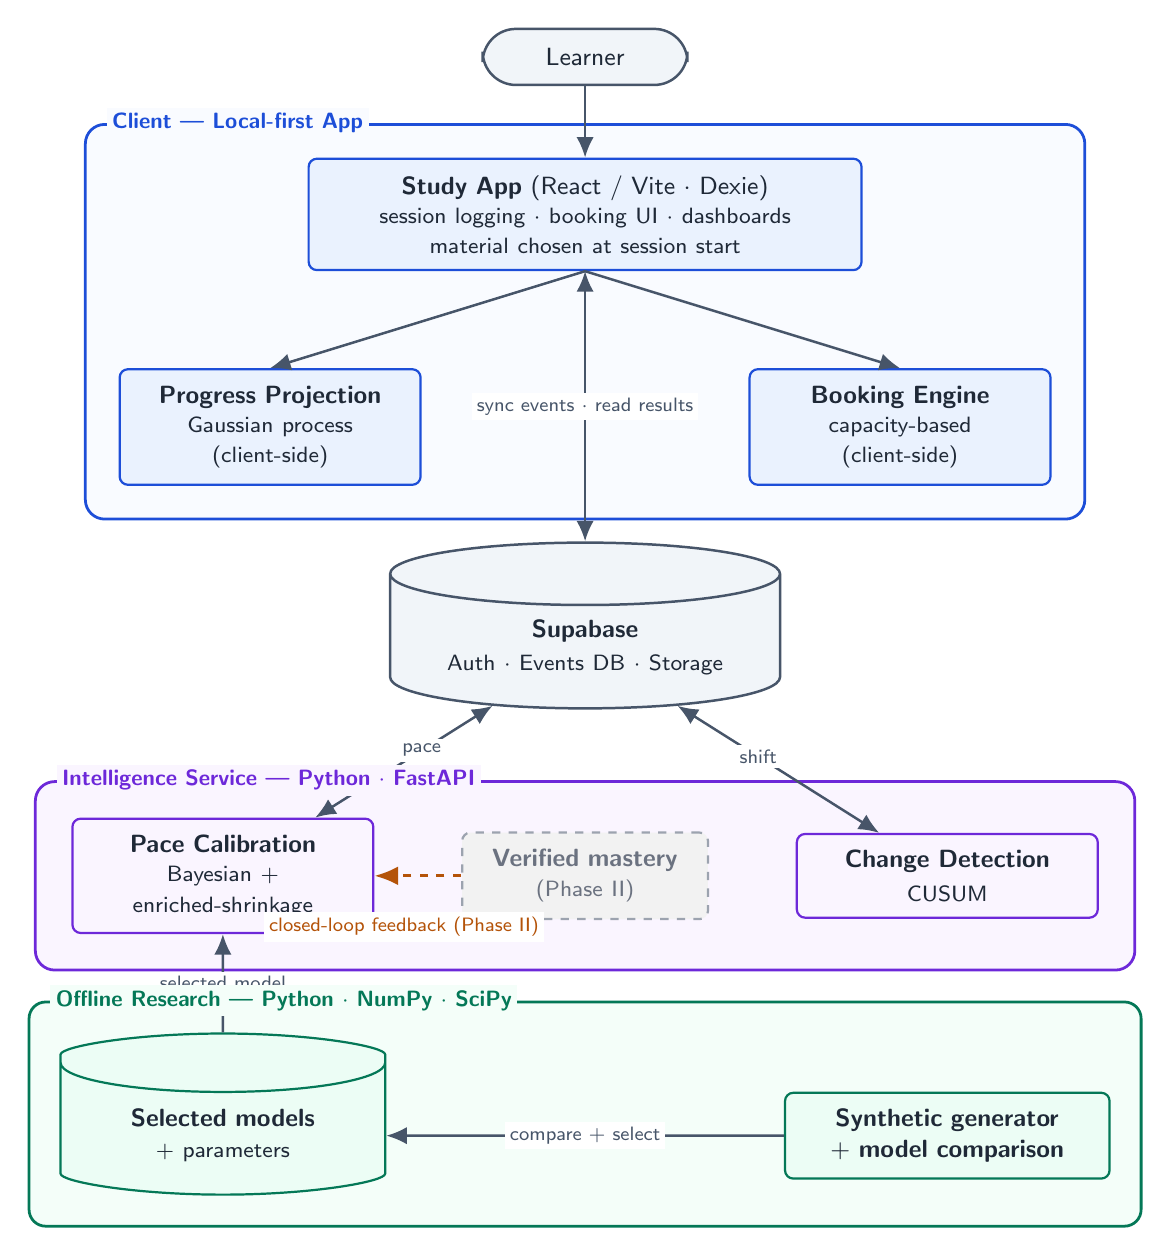
\begin{tikzpicture}[
  font=\small,
  every node/.style={text=inkText},
  box/.style={rounded corners=3pt, draw, line width=0.8pt, align=center,
              inner sep=6pt, text width=3.4cm, fill=white},
  proc/.style={box, draw=blueStroke, fill=paFill},
  svc/.style={box, draw=purpStroke, fill=purpFill},
  hub/.style={cylinder, shape border rotate=90, aspect=0.16, draw=slate,
              line width=0.9pt, fill=slateFill, align=center, inner sep=5pt,
              text width=4.6cm, minimum height=1.4cm},
  actor/.style={rounded corners=12pt, draw=slate, line width=0.9pt,
                fill=slateFill, align=center, inner sep=7pt, minimum width=2.6cm},
  res/.style={box, draw=greenStroke, fill=greenFill, text width=3.7cm},
  phase2/.style={rounded corners=3pt, draw=grey, dashed, line width=0.8pt,
                 fill=greyFill, text=greyText, align=center, inner sep=6pt, text width=2.7cm},
  title/.style={font=\footnotesize\bfseries},
  flow/.style={-{Latex[length=2.6mm,width=2.2mm]}, line width=0.9pt, draw=slate},
  flowbi/.style={{Latex[length=2.6mm,width=2.2mm]}-{Latex[length=2.6mm,width=2.2mm]},
                 line width=0.9pt, draw=slate},
  loop/.style={-{Latex[length=3.0mm,width=2.4mm]}, line width=1.1pt, dashed, draw=amber},
  lbl/.style={font=\scriptsize, fill=white, inner sep=1.8pt, text=slate},
  amblbl/.style={font=\scriptsize, fill=white, inner sep=1.8pt, text=amber},
]

% ---------------- NODES (absolute grid) ----------------
\node[actor] (LEARNER) at (2,16.4) {Learner};
\node[proc, text width=6.6cm] (APP) at (2,14.4)
  {\textbf{Study App} (React / Vite $\cdot$ Dexie)\\[1pt]\footnotesize session logging $\cdot$ booking UI $\cdot$ dashboards\\\footnotesize material chosen at session start};
\node[proc] (GP) at (-2.0,11.7) {\textbf{Progress Projection}\\[1pt]\footnotesize Gaussian process\\\footnotesize (client-side)};
\node[proc] (ENG) at (6.0,11.7) {\textbf{Booking Engine}\\[1pt]\footnotesize capacity-based\\\footnotesize (client-side)};

\node[hub] (SB) at (2,8.9) {\textbf{Supabase}\\[1pt]\footnotesize Auth $\cdot$ Events DB $\cdot$ Storage};

\node[svc] (CAL) at (-2.6,6.0) {\textbf{Pace Calibration}\\[1pt]\footnotesize Bayesian $+$\\\footnotesize enriched-shrinkage};
\node[phase2] (V2) at (2,6.0) {\textbf{Verified mastery}\\\footnotesize (Phase II)};
\node[svc] (DET) at (6.6,6.0) {\textbf{Change Detection}\\[1pt]\footnotesize CUSUM};

\node[res, cylinder, shape border rotate=90, aspect=0.18, minimum height=1.2cm] (MODELS)
  at (-2.6,2.7) {\textbf{Selected models}\\\footnotesize $+$ parameters};
\node[res] (PIPE) at (6.6,2.7) {\textbf{Synthetic generator}\\\textbf{$+$ model comparison}};

% ---------------- CONTAINERS (background) ----------------
\begin{scope}[on background layer]
  \node[draw=blueStroke, line width=1pt, rounded corners=7pt, fill=blueFill!40,
        fit=(APP)(GP)(ENG), inner sep=12pt] (clientBox) {};
  \node[draw=purpStroke, line width=1pt, rounded corners=7pt, fill=purpFill,
        fit=(CAL)(V2)(DET), inner sep=13pt] (svcBox) {};
  \node[draw=greenStroke, line width=1pt, rounded corners=6pt, fill=greenFill!60,
        fit=(MODELS)(PIPE), inner sep=11pt] (resBox) {};
\end{scope}

% ---------------- EDGES ----------------
\draw[flow] (LEARNER) -- (APP);
\draw[flow] (APP.south) -- (GP.north);
\draw[flow] (APP.south) -- (ENG.north);
\draw[flowbi] (APP) -- (SB) node[lbl, midway]{sync events $\cdot$ read results};
% Supabase <-> service (one /v1/calibration call; diverging clean edges)
\draw[flowbi] (SB) -- (CAL) node[lbl, pos=0.4]{pace};
\draw[flowbi] (SB) -- (DET) node[lbl, pos=0.4]{shift};
% research feeds the calibrator
\draw[flow] (PIPE) -- (MODELS) node[lbl, midway]{compare $+$ select};
\draw[flow] (MODELS) -- (CAL) node[lbl, midway]{selected model};
% closed loop (Phase II): verified mastery feeds calibration
\draw[loop] (V2.west) -- (CAL.east);
\node[amblbl] at (-0.3,5.35) {closed-loop feedback (Phase II)};

% ---------------- CONTAINER TITLES (on top) ----------------
\node[title, text=blueStroke, fill=blueFill!40, inner sep=2pt, anchor=west]
      at ([xshift=8pt]clientBox.north west) {Client --- Local-first App};
\node[title, text=purpStroke, fill=purpFill, inner sep=2pt, anchor=west]
      at ([xshift=8pt]svcBox.north west) {Intelligence Service --- Python $\cdot$ FastAPI};
\node[title, text=greenStroke, fill=greenFill!60, inner sep=2pt, anchor=west]
      at ([xshift=8pt]resBox.north west) {Offline Research --- Python $\cdot$ NumPy $\cdot$ SciPy};
\end{tikzpicture}
\end{document}
